\documentclass{article}


\usepackage{amsmath} % math stuff
\usepackage{amssymb} % math stuff
\usepackage{array} % equations and stuff
\usepackage{bm} % bold math
%\usepackage{caption} % suppressed table numbering; incompatible with revtex, and longtable, I think
\usepackage{comment} % comment environment
%\usepackage{enumitem} % customization of enumeration, itemize, and description
\usepackage[T1]{fontenc} % font encoding for special characters, must also use scalable font package
\usepackage[margin=0.8in]{geometry} % paper sizes and margins (but be careful not to mess up pre-defined pages)
\usepackage{graphicx} % for graphics
%\usepackage{helvet} % default font is the helvetica postscript font
\usepackage{lipsum} % lorem ipsum filler text
\usepackage{lmodern} % scalable font?
\usepackage{longtable} % multi-page tables
\usepackage{mathrsfs} % math script font
\usepackage{mhchem} % easier chemical formula
\usepackage{microtype} % allows disabling of ligatures
%\usepackage{newcent} % new century schoolbook font
\usepackage{nicefrac}
\usepackage{parskip} % removes paragraph indentation, and adjusts paragraph skip, as well as list items
%\usepackage{setspace} % adjust text spacing and indents
\usepackage{siunitx} % decimal alignment
\usepackage{subfigure} % divided figures
%\usepackage{tabu} % extra table options
\usepackage{textcomp} % symbols
\usepackage{threeparttablex} % better footnotes with longtable
\usepackage{titling} % title placement
\usepackage{ulem} % strikethrough text
%\usepackage{url} % superceded by hyperref
\usepackage{verbatim} % verbatim environment
\usepackage{xcolor} % colors and color boxes
\usepackage{xspace} % commands that don't eat up white space
\usepackage{hyperref} % links and page setup; should always come last

\hypersetup{
	bookmarks=true,
	colorlinks=true,
	citecolor=blue,
	linkcolor=blue,
	urlcolor=blue,
	pdfstartview={XYZ null null 1.0} % default open view is 100%
}

\DisableLigatures[f]{encoding = *, family = * } % disable ff, fi, fl ligatures, without f option, it also disables -- = endash
\renewcommand{\arraystretch}{1} % extra vertical space in tables

\begin{document}

\pagestyle{empty} % don't number pages

% custom title
\begin{center}
{\LARGE Classic Riddler}

\vspace{0.15in}

{\Large 31 January 2020}
\end{center}


\section*{Riddle:}

Robert’s daughter has a set of Magna-Tiles, which, as their name implies, are tiles with magnets on the edges that can be used to build various polygons and polyhedra.
Some of the tiles are identical isosceles triangles with one 30 degree angle and two 75 degree angles.
If you were to arrange 12 of these tiles with their 30 degree angles in the center, they would lay flat and form a regular dodecagon.
If you were to put fewer (between three and 11) of those tiles together in a similar way, they would form a pyramid whose base is a regular polygon.
Robert has graciously provided a photo of the resulting pyramids when three and 11 tiles are used:

\vspace{0.15in}
\begin{center}
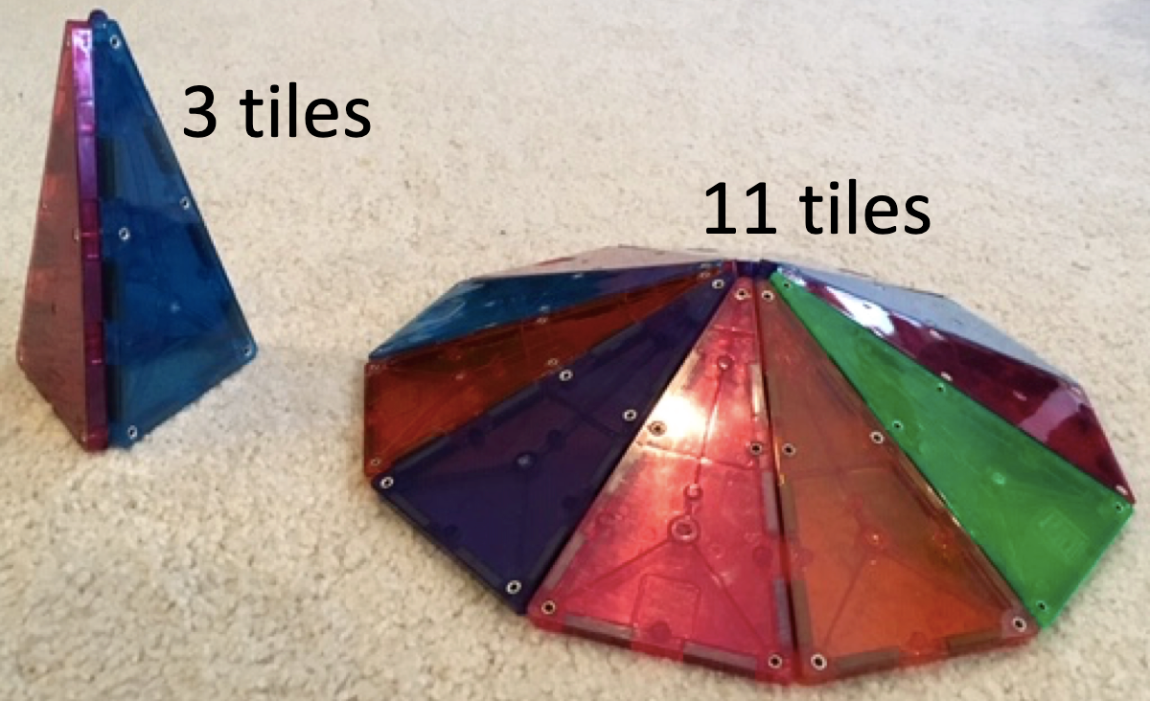
\includegraphics[width=3in]{pyramids.png}
\end{center}
\vspace{0.15in}

If Robert wanted to maximize the volume contained within the resulting pyramid (presumably to store as much candy for his daughter as possible), how many tiles should he use?

\section*{Solution:}

The general formula for the volume of a pyramid is $V=\nicefrac{1}{3}Bh$, where $B$ is the area of the base, and $h$ is the (perpendicular) height.
Of course, given a single tile, both of those must be determined individually for each pyramid.
To determine the values, I drew the following shapes:

\vspace{0.15in}
\begin{center}
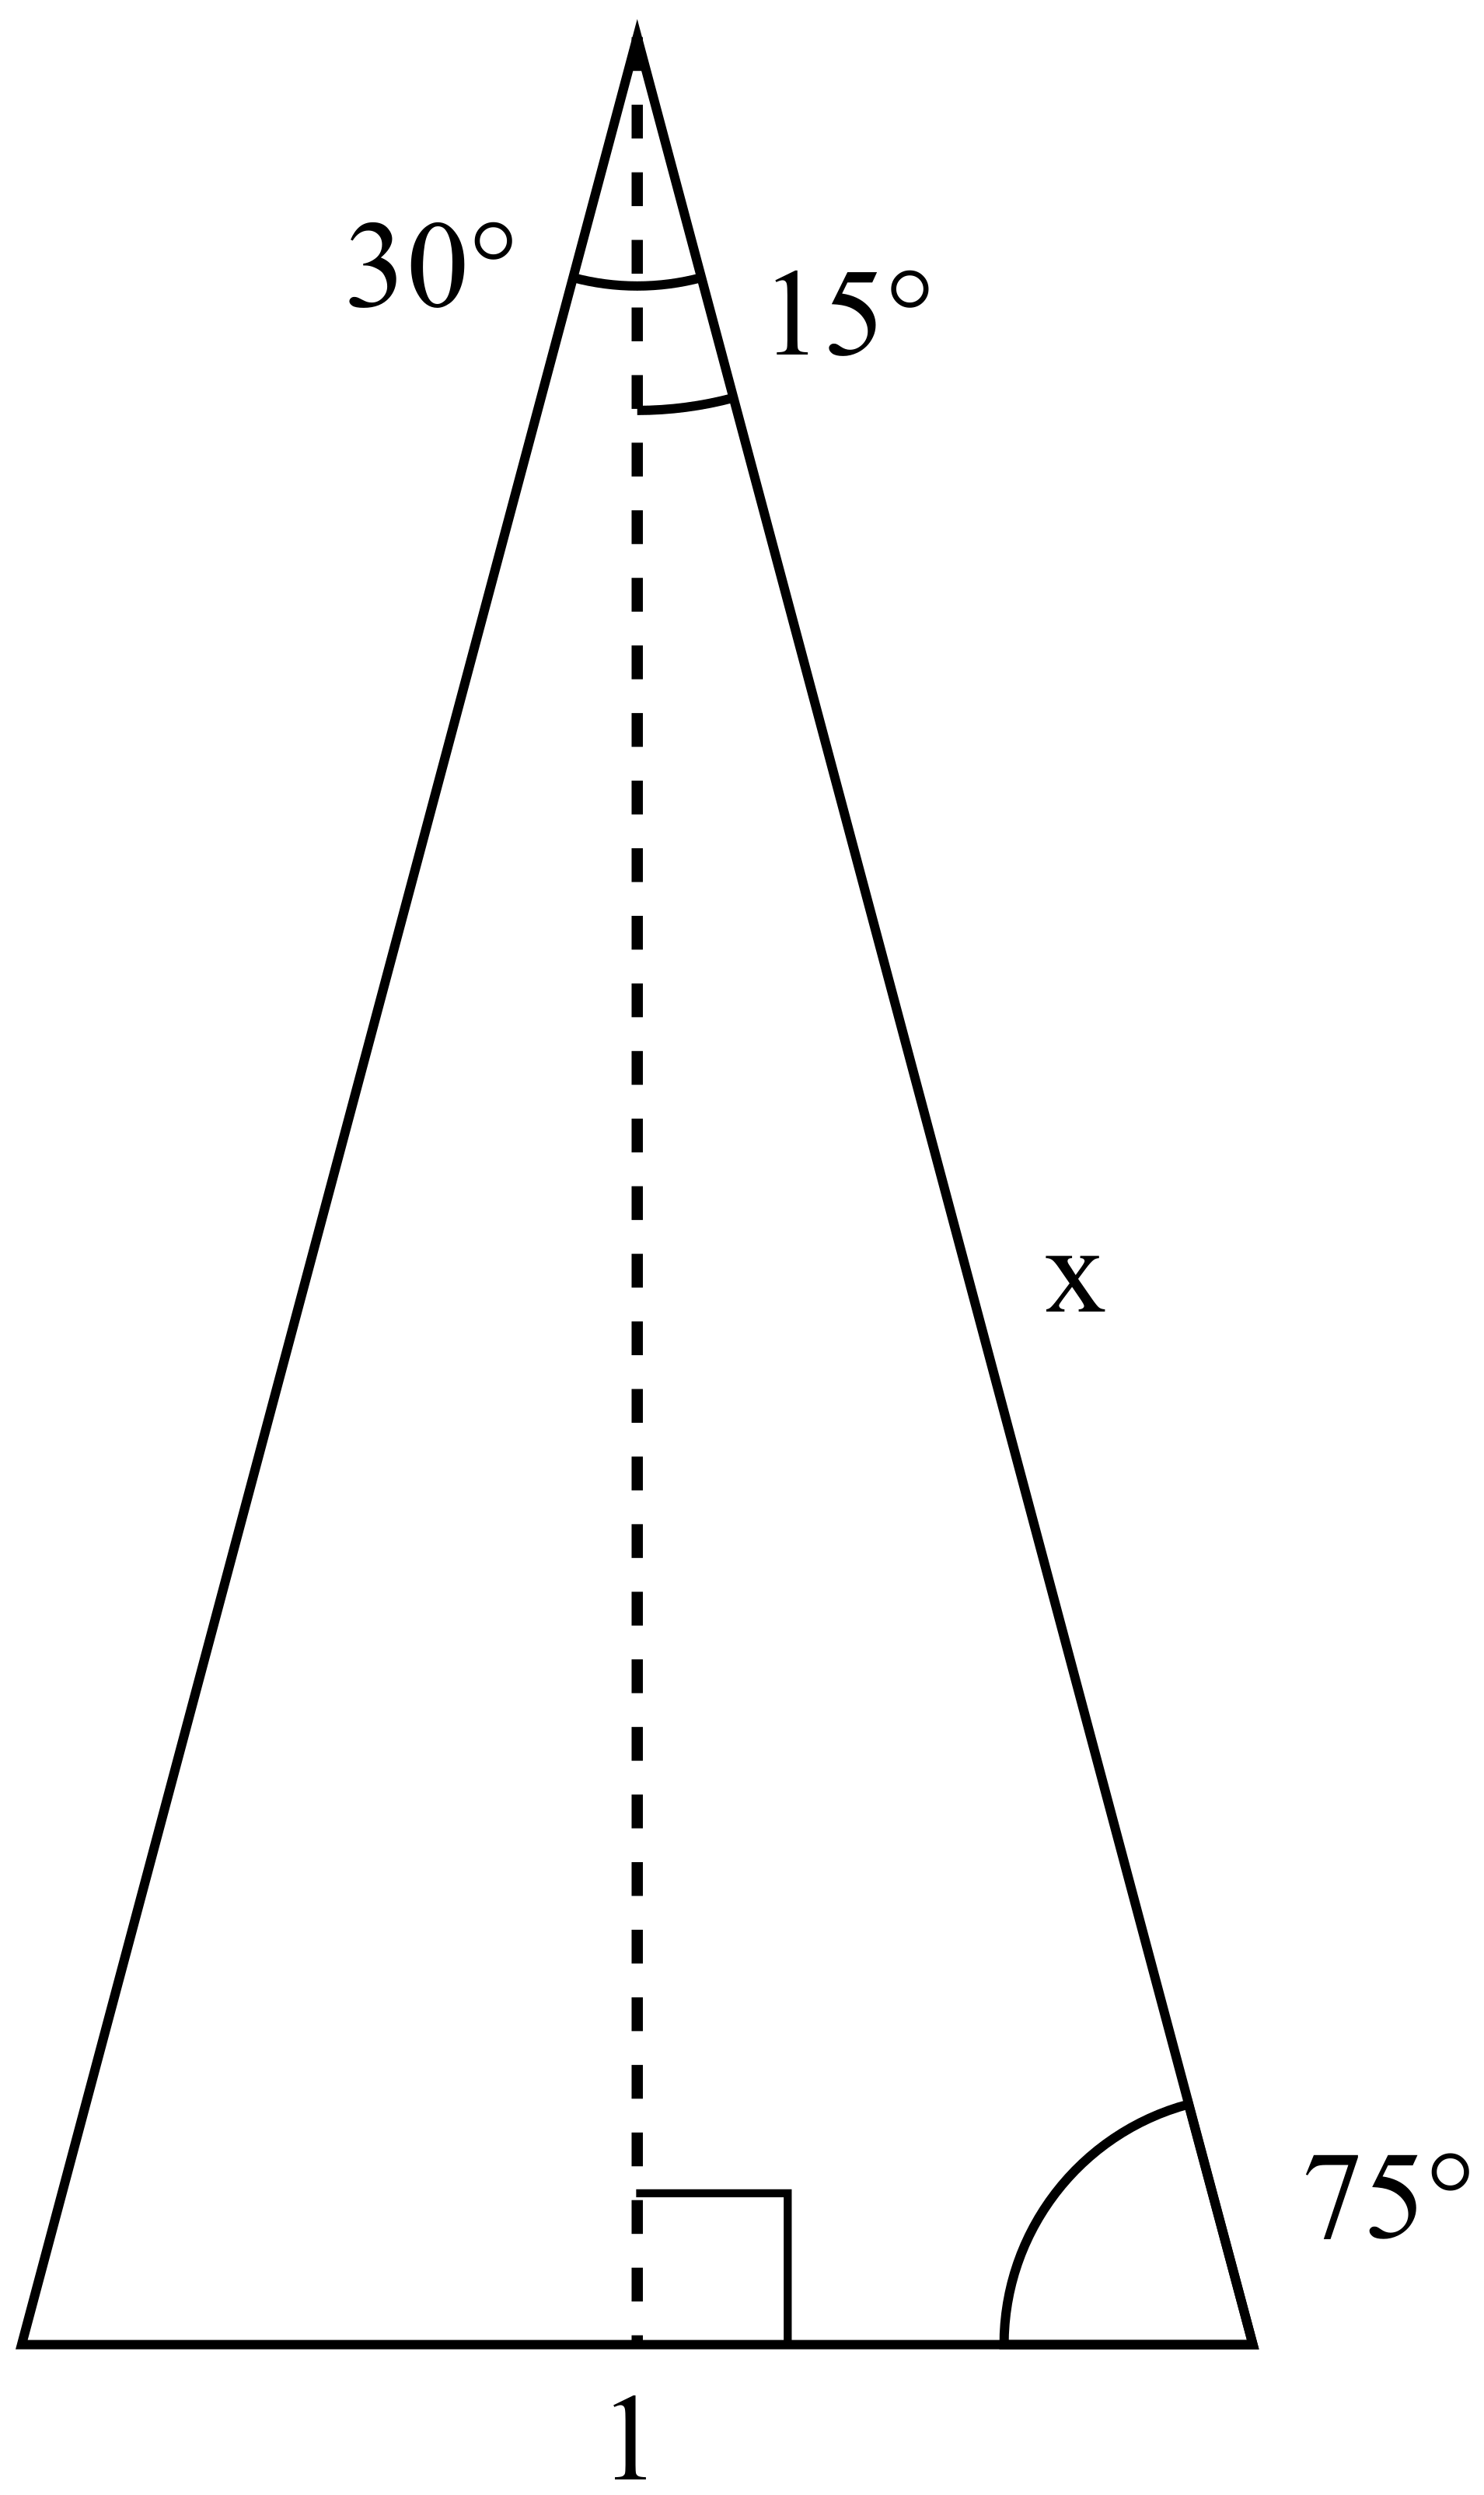
\includegraphics[scale=0.3]{triangle1.png}
\hspace{0.5in}
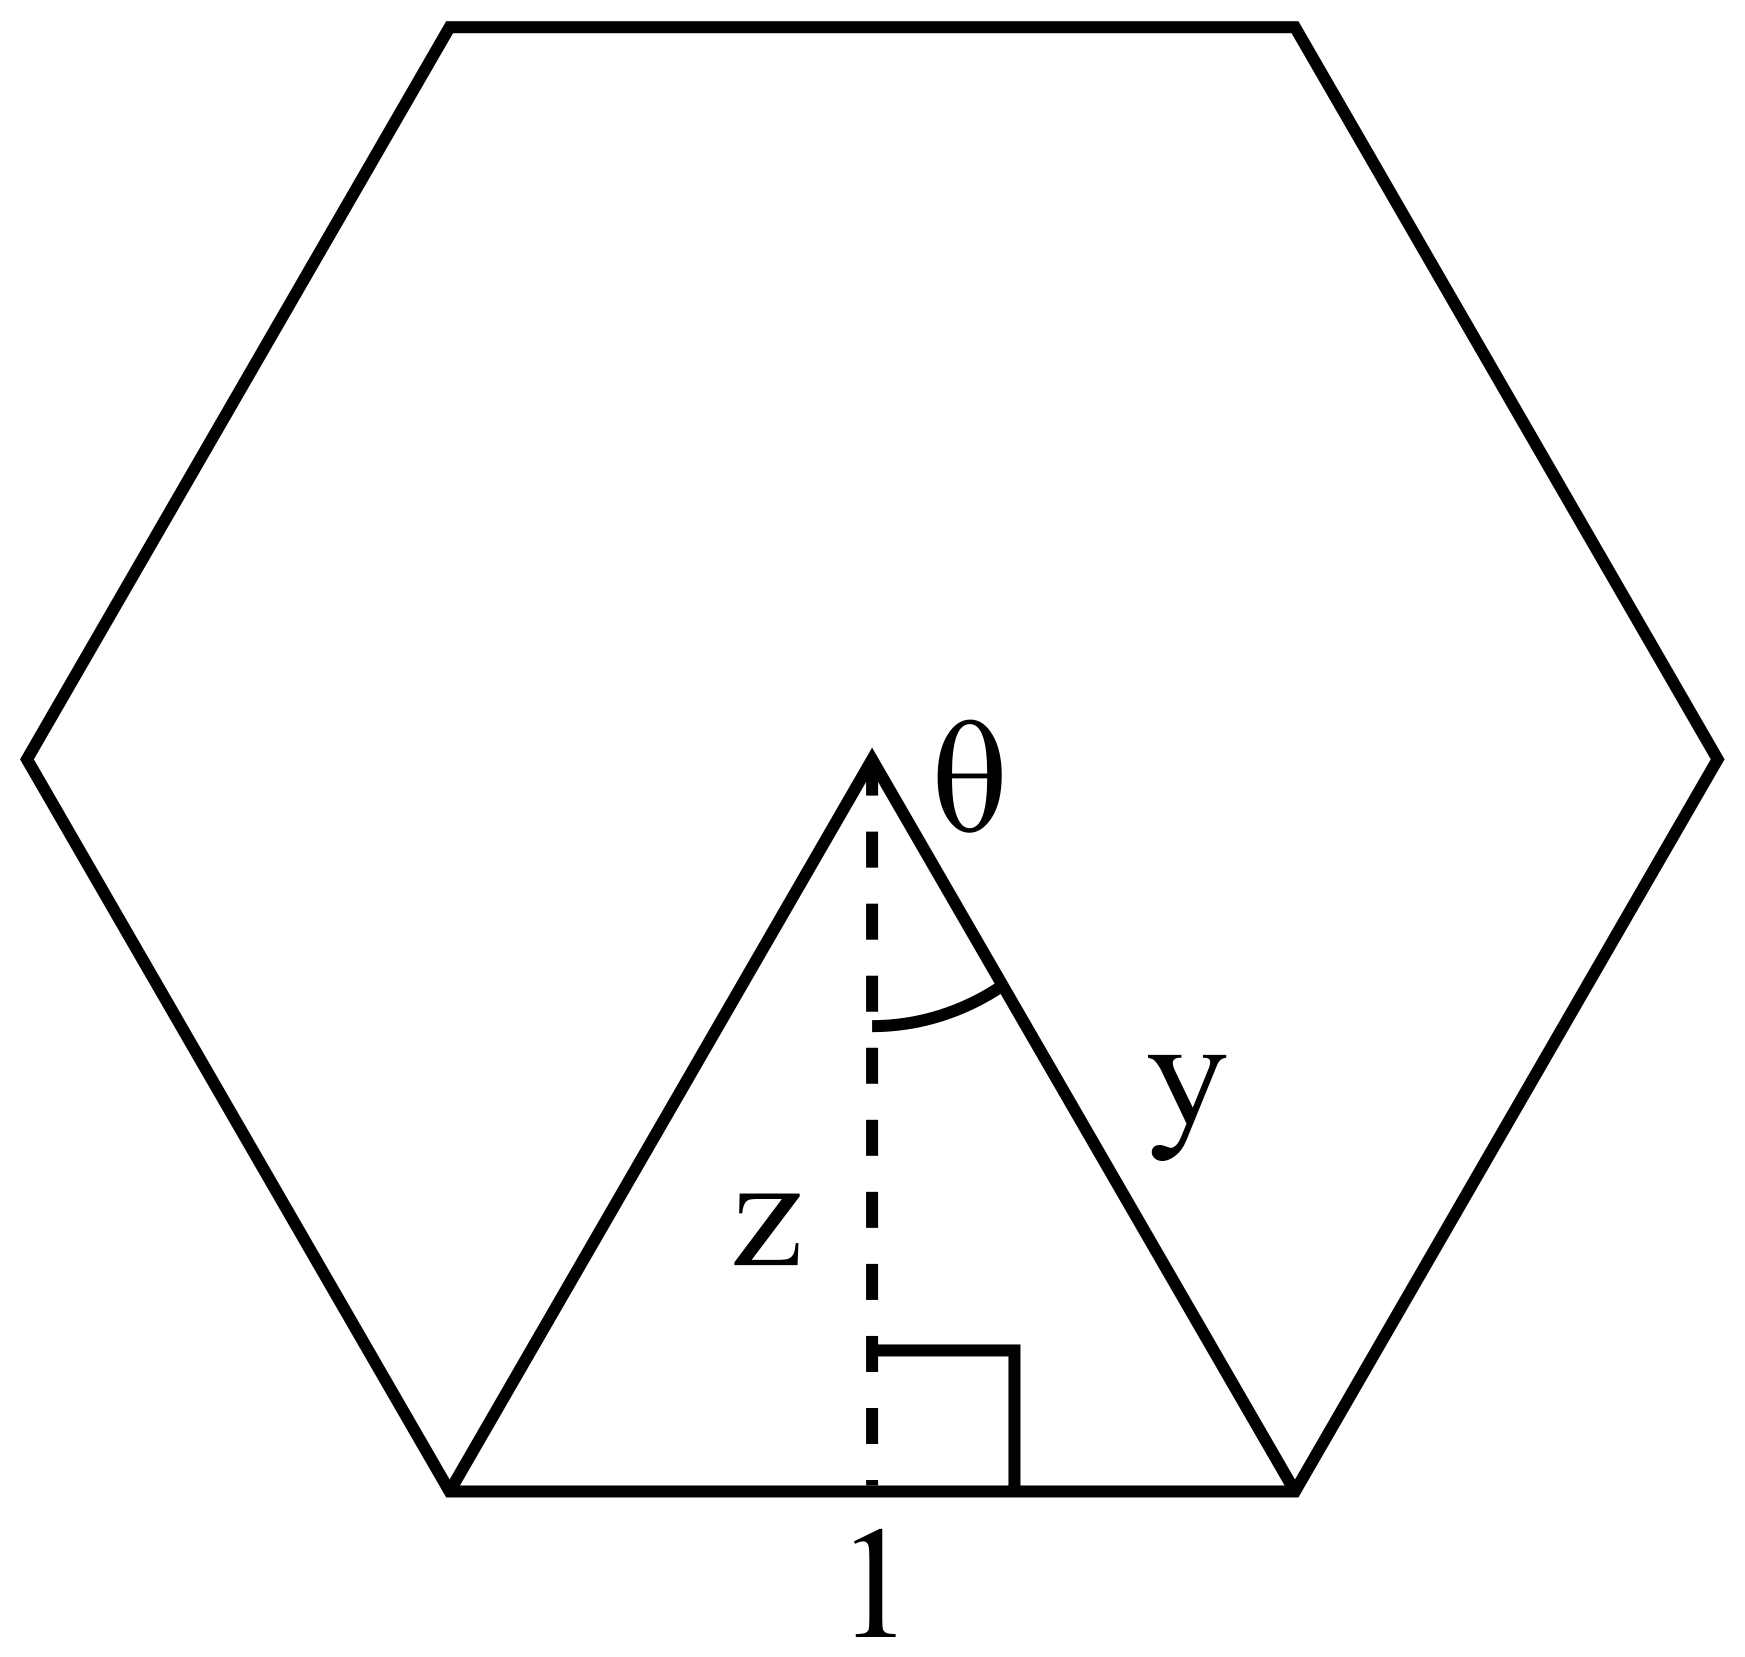
\includegraphics[scale=0.3]{polygon.png}
\hspace{0.5in}
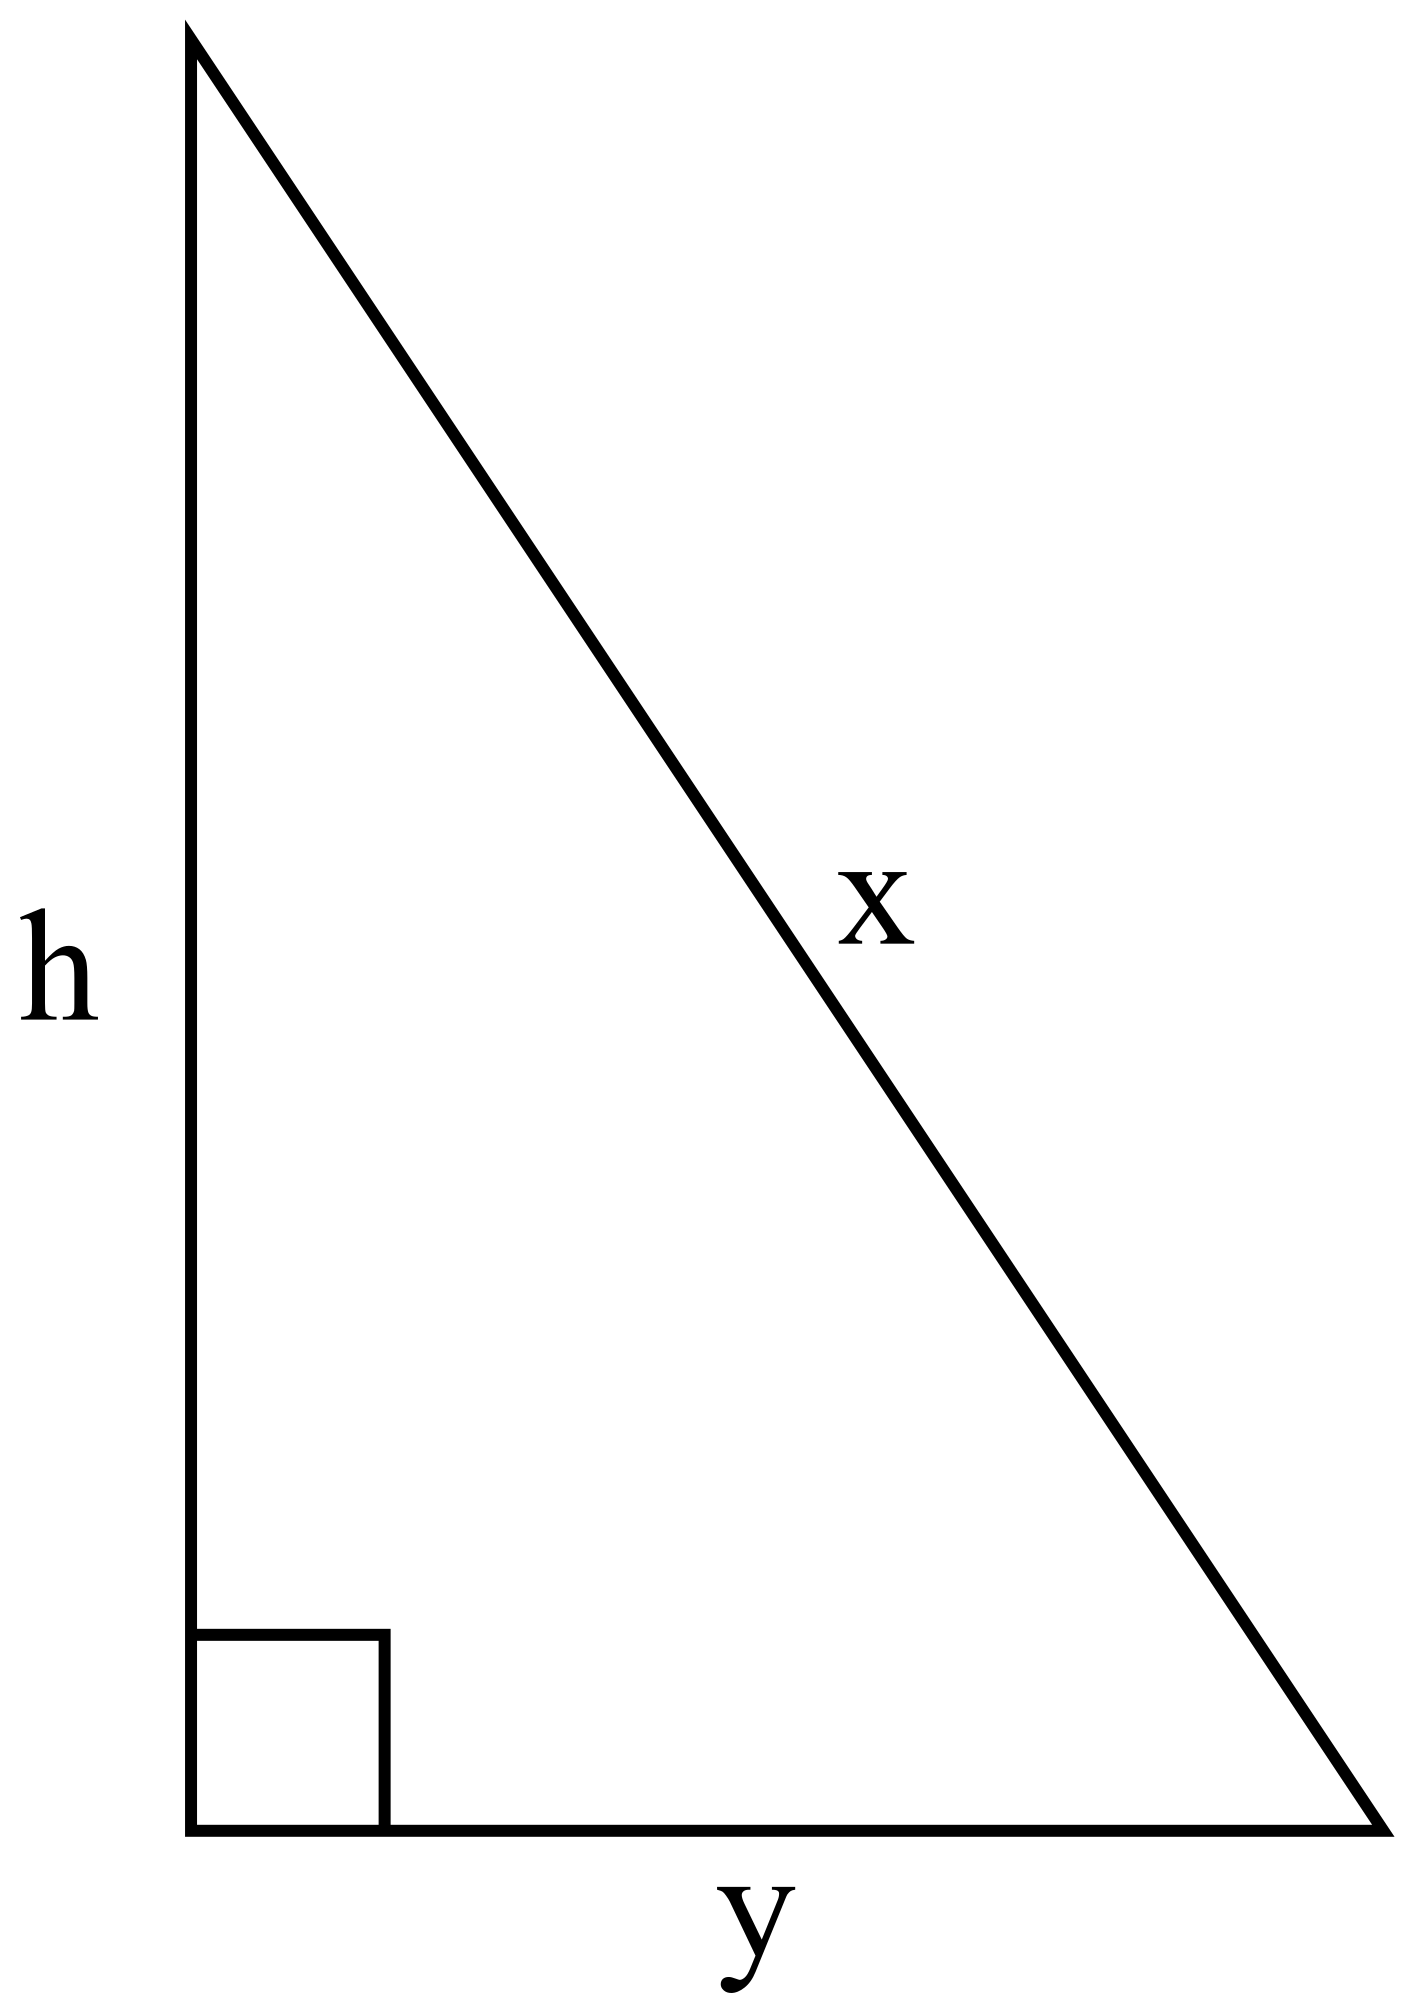
\includegraphics[scale=0.3]{triangle2.png}
\end{center}
\vspace{0.15in}

The first image is the given 75-75-30 tile.
Here I assigned the short side to be length 1.
Dividing it into two 75-15 right triangles, I get that each of the long sides must have length $x=\sqrt{2+\sqrt{3}}$, or about 1.931852.

Next I calculated the area of the base.
For $N$ pieces forming a regular $N$-gon, I divided the polygon into $N$ triangles, as seen in the center image.
These are the ``shadows'' of the tiles.
From the figure, it is clear that $\theta=\nicefrac{2\pi}{2N}=\nicefrac{\pi}{N}$.
Then, the area of each triangle is $A=\nicefrac{1}{2}\,z$, since the base of each triangle is 1.
Based on the right triangles, $z=\nicefrac{1}{2}\,\cot(\theta)$, so the area of each triangle is $A=\nicefrac{1}{4}\,\cot(\nicefrac{\pi}{N})$.
Because there are $N$ triangles in the $N$-gon, the total area of the pyramid's base is $B=\nicefrac{N}{4}\,\cot(\nicefrac{\pi}{N})$.

Next I calculated the height of the pyramid.
From the center image, $y=\nicefrac{1}{2}\,\csc(\theta)=\nicefrac{1}{2}\,\csc(\nicefrac{\pi}{N})$.
Then from the right image, the height is $h=\sqrt{x^{2}-y^{2}}$.
Combining all of these together, the volume of an $N$-sided pyramid is

\[
V(N)=\frac{1}{3}\frac{N}{4}\cot\left(\frac{\pi}{N}\right)\sqrt{\left(\sqrt{2+\sqrt{3}}\,\right)^{2}-\frac{\csc(\frac{\pi}{N})^{2}}{4}}
\]

Calculating this for up to 12 sides gives the following approximate values:

\vspace{0.15in}
\begin{center}
\begin{tabular*}{3.5in}{@{\extracolsep{\fill}} c c c c c}
N & V(N) & & N & V(N) \\
\cline{1-2} \cline{4-5}
1 & \textit{undefined} & & 7 & 1.8781 \\
2 & 0 & & 8 & 2.2903 \\
3 & 0.2661 & & 9 & 2.6023 \\
4 & 0.5993 & & 10 & 2.7070 \\
5 & 0.9947 & & 11 & 2.3824 \\
6 & 1.4314 & & 12 & 0
\end{tabular*}
\end{center}
\vspace{0.15in}

Therefore, the solution is
\fcolorbox{red}{white}{10 tiles}
with approximate volume
\fcolorbox{red}{white}{2.7070\dots}
(relative to each tile's short side).



\end{document}